\documentclass[12pt]{article}

\usepackage[margin=1in]{geometry}
\usepackage{amsmath}
\usepackage{amssymb}
\usepackage{amsthm}
\usepackage{mathrsfs}
\usepackage{mathtools}
\usepackage{tikz}
\usepackage[colorlinks=true, linkcolor=blue, bookmarks=true]{hyperref}

\title{\textbf{Rigorous Practice Problem Set: Divisibility, Logic, and Abstract Modeling}}
\author{Tashfeen Omran}
\date{October 2026}

\begin{document}

\maketitle

\tableofcontents
\newpage

\section{Concept Checklist \& Question Mapping}
\label{sec:checklist_start}
The following checklist details the theoretical concepts, logical structures, and proof techniques extracted from the source material, mapped directly to the problems in this document.

\begin{itemize}
    \item \textbf{C1: Direct Algebraic Manipulation \& Axioms of Divisibility} (Problems 1, 2, 3)
    \item \textbf{C2: Transitivity \& Linear Combinations} (Problems 4, 5)
    \item \textbf{C3: Biconditional Proofs ($\implies$ and $\impliedby$)} (Problems 6, 7)
    \item \textbf{C4: Proof by Cases / Division Algorithm} (Problems 8, 9, 10)
    \item \textbf{C5: Proof by Contrapositive \& De Morgan's Laws} (Problems 11, 12, 13)
    \item \textbf{C6: Parity Analysis of Products} (Problems 14, 15)
    \item \textbf{C7: Modular Arithmetic as a Filter (Squares mod 3, 4, 8)} (Problems 16, 17)
    \item \textbf{C8: B\'ezout's Identity \& Coprime Integers} (Problems 18, 19)
    \item \textbf{C9: Euclid's Lemma \& Prime Properties} (Problems 20, 21)
    \item \textbf{C10: Diagnostic Testing (Identifying Logical Flaws \& Fallacies)} (Problems 22, 23, 24, 25)
    \item \textbf{C11: Set-Theoretic Partitions \& Equivalence Relations} (Problems 26, 27)
    \item \textbf{C12: Abstract Real-World Modeling (Probability, ML, Quant Finance)} (Problems 28, 29)
    \item \textbf{C13: Advanced Conceptual Synthesis} (Problem 30)
\end{itemize}

\newpage

\section{Problem Set}

\subsection{Problem 1}
Let $a, b, c \in \mathbb{Z}$ with $a \neq 0$. Prove that if $a \mid b$ and $a \mid c$, then $a \mid (5b - 3c)$.

\subsection{Problem 2}
Let $a, b \in \mathbb{Z}$ with $a \neq 0$. Prove that if $a \mid b$, then $a^3 \mid b^3$.

\subsection{Problem 3}
Let $a, b, c, d \in \mathbb{Z}$ with $a \neq 0$. Prove that if $a \mid (b - c)$ and $a \mid (c - d)$, then $a \mid (b - d)$.

\subsection{Problem 4}
Let $a, b \in \mathbb{Z}$ with $a \neq 0$ and $b \neq 0$. Prove that if $a \mid b$ and $b \mid a$, then $a = b$ or $a = -b$.

\subsection{Problem 5}
Prove that for any integer $n$, $3 \mid (n^3 - n)$.

\subsection{Problem 6}
Let $n \in \mathbb{Z}$. Prove that $3 \mid (n^2 + 2)$ if and only if $3 \nmid n$.

\subsection{Problem 7}
Let $n \in \mathbb{Z}$. Prove that $n$ is odd if and only if $8 \mid (n^2 - 1)$.

\subsection{Problem 8}
Prove that the square of any integer is of the form $4k$ or $4k + 1$ for some $k \in \mathbb{Z}$.

\subsection{Problem 9}
Prove that for any integer $n$, $6 \mid n(n+1)(n+2)$.

\subsection{Problem 10}
Prove that there are no integers $x$ and $y$ such that $x^2 - 4y = 2$.

\subsection{Problem 11}
Prove by contrapositive: For any integers $a$ and $b$, if $5 \nmid ab$, then $5 \nmid a$ and $5 \nmid b$.

\subsection{Problem 12}
Prove by contrapositive: For any integer $n$, if $n^3$ is even, then $n$ is even.

\subsection{Problem 13}
Prove by contrapositive: Let $a, b, c \in \mathbb{Z}$. If $a^2 + b^2 = c^2$, then $3 \mid a$ or $3 \mid b$.

\subsection{Problem 14}
Let $n \in \mathbb{Z}$. Prove that if $n$ is an odd integer, then $n^4 \equiv 1 \pmod{16}$.

\subsection{Problem 15}
Let $n \in \mathbb{Z}$. Prove that if $3 \nmid n$, then $n^2 \equiv 1 \pmod 3$.

\subsection{Problem 16}
Let $a, b \in \mathbb{Z}$. Prove that if $\gcd(a, b) = 1$ and $a \mid bc$, then $a \mid c$.

\subsection{Problem 17}
Let $a, b, c \in \mathbb{Z}$. Prove that if $a \mid c$ and $b \mid c$, and $\gcd(a, b) = 1$, then $ab \mid c$.

\subsection{Problem 18}
Prove that for any integer $n$, $\gcd(n, n+1) = 1$.

\subsection{Problem 19}
Let $p$ be a prime number and $a \in \mathbb{Z}$. Prove that if $p \mid a^2$, then $p \mid a$.

\subsection{Problem 20}
Find a counterexample to the following claim: ``For all integers $a, b, c$, if $a \mid c$ and $b \mid c$, then $ab \mid c$.''

\subsection{Problem 21}
Identify the fatal logical flaw in the following proof:
\textit{Claim:} If $a \mid (b+c)$, then $a \mid b$ or $a \mid c$.
\textit{Proof:} Assume $a \mid (b+c)$. By definition, $b+c = ak$ for some $k \in \mathbb{Z}$. We can write $k = k_1 + k_2$. Thus, $b+c = a(k_1 + k_2) = ak_1 + ak_2$. Matching terms, $b = ak_1$ and $c = ak_2$. Therefore, $a \mid b$ and $a \mid c$, which implies $a \mid b$ or $a \mid c$.

\subsection{Problem 22}
Identify the fatal logical flaw in the following proof:
\textit{Claim:} If $x^2 \equiv 0 \pmod 4$, then $x \equiv 0 \pmod 4$.
\textit{Proof:} Assume $x^2 \equiv 0 \pmod 4$. This means $4 \mid x^2$, which is $4 \mid (x \cdot x)$. By the property of divisibility, if a number divides a product, it must divide one of the factors. Therefore, $4 \mid x$ or $4 \mid x$. In either case, $4 \mid x$, so $x \equiv 0 \pmod 4$.

\subsection{Problem 23}
Find a counterexample to the following claim: ``If $a \mid b^2$, then $a \mid b$.''

\subsection{Problem 24}
Identify the fatal logical flaw in the following proof:
\textit{Claim:} If $a \mid b$, then $a \mid bc$.
\textit{Proof:} Assume $a \mid b$. Then $\frac{b}{a} = k$ for some integer $k$. Multiply both sides by $c$ to get $\frac{bc}{a} = kc$. Since $k$ and $c$ are integers, $kc$ is an integer. Therefore, $a \mid bc$.

\subsection{Problem 25}
Establish the logical equivalence of the following two statements for $a, b \in \mathbb{Z}$:
(1) $a \mid b$
(2) $b \mathbb{Z} \subseteq a \mathbb{Z}$

\subsection{Problem 26}
Let $A = 3\mathbb{Z}$ and $B = 5\mathbb{Z}$. Prove set-theoretically that $A \cap B = 15\mathbb{Z}$.

\subsection{Problem 27}
Define a relation $\sim$ on $\mathbb{Z}$ by $x \sim y \iff 4 \mid (x - y)$. Prove that $\sim$ is an equivalence relation.

\subsection{Problem 28}
\textbf{(Distributed ML Load Balancing)} Let the state space of training data indices be $\Omega = \{1, 2, \dots, 1000\}$. We define a probability space $(\Omega, \mathscr{F}, \mathbb{P})$ where each index is chosen uniformly at random. A hash function $X: \Omega \to \{0, 1, 2, 3, 4\}$ routes data to 5 GPUs based on the rule $X(\omega) = \omega \bmod 5$. Derive the exact probability measure $\mathbb{P}(X = i)$ for all $i \in \{0, 1, 2, 3, 4\}$ and prove that the load is perfectly uniformly distributed.

\subsection{Problem 29}
\textbf{(Algorithmic Trading Time-Series)} High-frequency timestamps $T_1, T_2, T_3 \in \mathbb{Z}$ are aligned into discrete buckets of size $\Delta t \in \mathbb{Z}^+$. Two timestamps belong to the same bucket if they are congruent modulo $\Delta t$. Prove that if $T_1$ and $T_2$ are in the same bucket, and $T_2$ and $T_3$ are in the same bucket, then $T_1$ and $T_3$ must be in the same bucket.

\subsection{Problem 30}
\textbf{(Advanced Conceptual Synthesis)} Let $p$ be a prime number strictly greater than 3. Prove that $24 \mid (p^2 - 1)$. \textit{(Hint: Synthesize parity analysis, modular arithmetic filters, and coprime divisibility theorems).}

\newpage

\section{Detailed Solutions}

\subsection{Solution to Problem 1}
\begin{proof}
\textbf{Proof Technique: Direct Proof (Linear Combination).} \\
Assume $a \mid b$ and $a \mid c$. By the definition of divisibility, there exist integers $k_1, k_2 \in \mathbb{Z}$ such that $b = ak_1$ and $c = ak_2$. We wish to show that $a \mid (5b - 3c)$. We substitute our expressions for $b$ and $c$ into the target expression:
\[ 5b - 3c = 5(ak_1) - 3(ak_2) \]
Factoring out $a$, we obtain:
\[ 5b - 3c = a(5k_1 - 3k_2) \]
Since $k_1, k_2 \in \mathbb{Z}$, and the integers are closed under multiplication and subtraction, let $m = 5k_1 - 3k_2$ where $m \in \mathbb{Z}$. Thus, $5b - 3c = am$. By definition, this implies $a \mid (5b - 3c)$.
\end{proof}

\subsection{Solution to Problem 2}
\begin{proof}
\textbf{Proof Technique: Direct Proof.} \\
Assume $a \mid b$. By definition, there exists an integer $k \in \mathbb{Z}$ such that $b = ak$. We wish to show that $a^3 \mid b^3$. Cubing both sides of the equation yields:
\[ b^3 = (ak)^3 = a^3 k^3 \]
Since $k \in \mathbb{Z}$ and integers are closed under multiplication, $k^3 \in \mathbb{Z}$. Let $m = k^3$. Then $b^3 = a^3 m$. By definition, $a^3 \mid b^3$.
\end{proof}

\subsection{Solution to Problem 3}
\begin{proof}
\textbf{Proof Technique: Direct Proof.} \\
Assume $a \mid (b - c)$ and $a \mid (c - d)$. By definition, there exist integers $k_1, k_2 \in \mathbb{Z}$ such that:
\[ b - c = ak_1 \]
\[ c - d = ak_2 \]
We wish to show $a \mid (b - d)$. Adding the two equations together yields:
\[ (b - c) + (c - d) = ak_1 + ak_2 \]
\[ b - d = a(k_1 + k_2) \]
Since $k_1, k_2 \in \mathbb{Z}$, their sum $m = k_1 + k_2 \in \mathbb{Z}$. Thus, $b - d = am$, which implies $a \mid (b - d)$.
\end{proof}

\subsection{Solution to Problem 4}
\begin{proof}
\textbf{Proof Technique: Direct Proof.} \\
Assume $a \mid b$ and $b \mid a$. By definition, there exist integers $k_1, k_2 \in \mathbb{Z}$ such that $b = ak_1$ and $a = bk_2$. Substituting the first equation into the second yields:
\[ a = (ak_1)k_2 = a(k_1 k_2) \]
Since $a \neq 0$, we can divide both sides by $a$ (or formally, $a - a(k_1 k_2) = 0 \implies a(1 - k_1 k_2) = 0 \implies 1 - k_1 k_2 = 0$ since $a \neq 0$). This gives:
\[ k_1 k_2 = 1 \]
Since $k_1, k_2 \in \mathbb{Z}$, the only integer solutions to this product are $k_1 = 1, k_2 = 1$ or $k_1 = -1, k_2 = -1$. 
If $k_1 = 1$, then $b = a(1) \implies a = b$. 
If $k_1 = -1$, then $b = a(-1) \implies a = -b$. 
Thus, $a = b$ or $a = -b$.
\end{proof}

\subsection{Solution to Problem 5}
\begin{proof}
\textbf{Proof Technique: Direct Proof by Factoring and Cases.} \\
Let $n \in \mathbb{Z}$. We wish to show $3 \mid (n^3 - n)$. First, we factor the expression:
\[ n^3 - n = n(n^2 - 1) = n(n - 1)(n + 1) = (n - 1)n(n + 1) \]
This is the product of three consecutive integers. By the Division Algorithm, any integer $n$ can be expressed as $3k, 3k+1,$ or $3k+2$ for some $k \in \mathbb{Z}$.
\textbf{Case 1:} $n = 3k$. Then the factor $n$ is divisible by 3, making the entire product divisible by 3.
\textbf{Case 2:} $n = 3k + 1$. Then the factor $(n - 1) = 3k$, which is divisible by 3, making the product divisible by 3.
\textbf{Case 3:} $n = 3k + 2$. Then the factor $(n + 1) = 3k + 3 = 3(k + 1)$, which is divisible by 3, making the product divisible by 3.
In all cases, one of the factors is a multiple of 3. Thus, $3 \mid (n^3 - n)$.
\end{proof}

\subsection{Solution to Problem 6}
\begin{proof}
\textbf{Proof Technique: Biconditional Proof.} \\
We must prove both directions: $3 \mid (n^2 + 2) \implies 3 \nmid n$ and $3 \nmid n \implies 3 \mid (n^2 + 2)$.
\textbf{Part 1 ($\implies$):} We prove the contrapositive: If $3 \mid n$, then $3 \nmid (n^2 + 2)$. Assume $3 \mid n$. Then $n = 3k$ for some $k \in \mathbb{Z}$. Substituting this into $n^2 + 2$:
\[ n^2 + 2 = (3k)^2 + 2 = 9k^2 + 2 = 3(3k^2) + 2 \]
Since $3k^2 \in \mathbb{Z}$, the Division Algorithm states the remainder is 2 when divided by 3. Thus, $3 \nmid (n^2 + 2)$.
\textbf{Part 2 ($\impliedby$):} We use a direct proof by cases. Assume $3 \nmid n$. By the Division Algorithm, $n = 3k + 1$ or $n = 3k + 2$.
\textit{Case 1:} $n = 3k + 1$. Then $n^2 + 2 = (3k + 1)^2 + 2 = 9k^2 + 6k + 1 + 2 = 9k^2 + 6k + 3 = 3(3k^2 + 2k + 1)$. Since $(3k^2 + 2k + 1) \in \mathbb{Z}$, $3 \mid (n^2 + 2)$.
\textit{Case 2:} $n = 3k + 2$. Then $n^2 + 2 = (3k + 2)^2 + 2 = 9k^2 + 12k + 4 + 2 = 9k^2 + 12k + 6 = 3(3k^2 + 4k + 2)$. Since $(3k^2 + 4k + 2) \in \mathbb{Z}$, $3 \mid (n^2 + 2)$.
Since both directions hold, the biconditional is proven.
\end{proof}

\subsection{Solution to Problem 7}
\begin{proof}
\textbf{Proof Technique: Biconditional Proof.} \\
\textbf{Part 1 ($\implies$):} Assume $n$ is odd. Then $n = 2k + 1$ for some $k \in \mathbb{Z}$. We evaluate $n^2 - 1$:
\[ n^2 - 1 = (2k + 1)^2 - 1 = 4k^2 + 4k + 1 - 1 = 4k^2 + 4k = 4k(k + 1) \]
Notice that $k(k + 1)$ is the product of two consecutive integers. One of them must be even, so $k(k + 1) = 2m$ for some $m \in \mathbb{Z}$. Substituting this back yields:
\[ n^2 - 1 = 4(2m) = 8m \]
Thus, $8 \mid (n^2 - 1)$.
\textbf{Part 2 ($\impliedby$):} We prove the contrapositive: If $n$ is even, then $8 \nmid (n^2 - 1)$. Assume $n$ is even. Then $n = 2k$ for some $k \in \mathbb{Z}$. We evaluate $n^2 - 1$:
\[ n^2 - 1 = (2k)^2 - 1 = 4k^2 - 1 \]
Since $4k^2$ is even, $4k^2 - 1$ is odd. An even number (8) cannot divide an odd number. Thus, $8 \nmid (n^2 - 1)$.
Both directions are proven.
\end{proof}

\subsection{Solution to Problem 8}
\begin{proof}
\textbf{Proof Technique: Proof by Cases (Parity).} \\
Let $n \in \mathbb{Z}$. By the Division Algorithm, $n$ is either even ($n = 2k$) or odd ($n = 2k + 1$) for some $k \in \mathbb{Z}$.
\textbf{Case 1:} $n$ is even. Then $n = 2k$. Squaring $n$ yields:
\[ n^2 = (2k)^2 = 4k^2 \]
Let $m = k^2 \in \mathbb{Z}$. Then $n^2 = 4m$, which is of the form $4m$.
\textbf{Case 2:} $n$ is odd. Then $n = 2k + 1$. Squaring $n$ yields:
\[ n^2 = (2k + 1)^2 = 4k^2 + 4k + 1 = 4(k^2 + k) + 1 \]
Let $m = k^2 + k \in \mathbb{Z}$. Then $n^2 = 4m + 1$, which is of the form $4m + 1$.
Since these cases exhaust all integers, the square of any integer is of the form $4k$ or $4k + 1$.
\end{proof}

\subsection{Solution to Problem 9}
\begin{proof}
\textbf{Proof Technique: Direct Proof (Divisibility by Coprimes).} \\
Let $E = n(n+1)(n+2)$. This is the product of three consecutive integers. 
First, at least one of $n, n+1, n+2$ must be even. Therefore, $2 \mid E$.
Second, exactly one of $n, n+1, n+2$ must be a multiple of 3 (by the Division Algorithm, the remainders modulo 3 cycle $0, 1, 2$). Therefore, $3 \mid E$.
Since $2 \mid E$ and $3 \mid E$, and $\gcd(2, 3) = 1$, it follows by the property of coprime divisors (proven in Problem 17) that $(2 \times 3) \mid E$. Thus, $6 \mid n(n+1)(n+2)$.
\end{proof}

\subsection{Solution to Problem 10}
\begin{proof}
\textbf{Proof Technique: Proof by Contradiction (Parity/Modular Arithmetic).} \\
Assume, for the sake of contradiction, that there exist integers $x, y \in \mathbb{Z}$ such that $x^2 - 4y = 2$. Rearranging the equation yields:
\[ x^2 = 4y + 2 = 2(2y + 1) \]
Since $2y + 1 \in \mathbb{Z}$, $x^2$ is an even integer. If $x^2$ is even, then $x$ must be even. Let $x = 2k$ for some $k \in \mathbb{Z}$. Substitute this back into the equation:
\[ (2k)^2 = 4y + 2 \]
\[ 4k^2 = 4y + 2 \]
Divide the entire equation by 2:
\[ 2k^2 = 2y + 1 \]
The left side, $2k^2$, is an even integer. The right side, $2y + 1$, is an odd integer. An even integer cannot equal an odd integer. This is a contradiction. Therefore, no such integers $x, y$ exist.
\end{proof}

\subsection{Solution to Problem 11}
\begin{proof}
\textbf{Proof Technique: Proof by Contrapositive \& De Morgan's Laws.} \\
The statement is of the form $P \implies (Q \land R)$. The contrapositive is $\neg(Q \land R) \implies \neg P$, which by De Morgan's Laws is $(\neg Q \lor \neg R) \implies \neg P$.
Thus, we must prove: If $5 \mid a$ or $5 \mid b$, then $5 \mid ab$.
Assume $5 \mid a$ or $5 \mid b$. Without loss of generality, assume $5 \mid a$. By definition, $a = 5k$ for some $k \in \mathbb{Z}$. We evaluate the product $ab$:
\[ ab = (5k)b = 5(kb) \]
Since $k, b \in \mathbb{Z}$, their product $kb \in \mathbb{Z}$. Let $m = kb$. Then $ab = 5m$, which implies $5 \mid ab$. (The proof is identical if we assume $5 \mid b$). This proves the contrapositive, and thus the original statement is true.
\end{proof}

\subsection{Solution to Problem 12}
\begin{proof}
\textbf{Proof Technique: Proof by Contrapositive.} \\
We must prove: If $n$ is odd, then $n^3$ is odd.
Assume $n$ is odd. By definition, $n = 2k + 1$ for some $k \in \mathbb{Z}$. We evaluate $n^3$:
\[ n^3 = (2k + 1)^3 = 8k^3 + 12k^2 + 6k + 1 \]
We can factor out a 2 from the first three terms:
\[ n^3 = 2(4k^3 + 6k^2 + 3k) + 1 \]
Since $k \in \mathbb{Z}$, the expression $m = 4k^3 + 6k^2 + 3k$ is an integer due to closure under addition and multiplication. Thus, $n^3 = 2m + 1$, which means $n^3$ is odd. This completes the proof by contrapositive.
\end{proof}

\subsection{Solution to Problem 13}
\begin{proof}
\textbf{Proof Technique: Proof by Contrapositive (Modular Arithmetic Filter).} \\
We must prove: If $3 \nmid a$ and $3 \nmid b$, then $a^2 + b^2 \neq c^2$.
Assume $3 \nmid a$ and $3 \nmid b$. By Problem 15, the square of any integer not divisible by 3 has a remainder of 1 when divided by 3. Therefore:
\[ a^2 \equiv 1 \pmod 3 \]
\[ b^2 \equiv 1 \pmod 3 \]
Adding these congruences yields:
\[ a^2 + b^2 \equiv 1 + 1 \equiv 2 \pmod 3 \]
This means $a^2 + b^2$ is of the form $3k + 2$. However, $c$ is an integer, and the square of any integer $c^2$ can only be congruent to $0$ or $1 \pmod 3$. Since $c^2$ can never have a remainder of 2 modulo 3, it is impossible for $a^2 + b^2 = c^2$. Thus, $a^2 + b^2 \neq c^2$.
\end{proof}

\subsection{Solution to Problem 14}
\begin{proof}
\textbf{Proof Technique: Direct Proof.} \\
Assume $n$ is an odd integer. From Problem 7, we established that if $n$ is odd, $8 \mid (n^2 - 1)$. This means $n^2 - 1 = 8k$ for some $k \in \mathbb{Z}$, or equivalently, $n^2 = 8k + 1$.
We wish to evaluate $n^4 \pmod{16}$. We square $n^2$:
\[ n^4 = (n^2)^2 = (8k + 1)^2 = 64k^2 + 16k + 1 \]
Factor out 16 from the first two terms:
\[ n^4 = 16(4k^2 + k) + 1 \]
Since $4k^2 + k \in \mathbb{Z}$, let $m = 4k^2 + k$. Then $n^4 = 16m + 1$. By the definition of congruence, $n^4 \equiv 1 \pmod{16}$.
\end{proof}

\subsection{Solution to Problem 15}
\begin{proof}
\textbf{Proof Technique: Proof by Cases.} \\
Assume $3 \nmid n$. By the Division Algorithm, $n$ must be of the form $3k + 1$ or $3k + 2$ for some $k \in \mathbb{Z}$.
\textbf{Case 1:} $n = 3k + 1$.
\[ n^2 = (3k + 1)^2 = 9k^2 + 6k + 1 = 3(3k^2 + 2k) + 1 \]
Since $3k^2 + 2k \in \mathbb{Z}$, $n^2 \equiv 1 \pmod 3$.
\textbf{Case 2:} $n = 3k + 2$.
\[ n^2 = (3k + 2)^2 = 9k^2 + 12k + 4 = 9k^2 + 12k + 3 + 1 = 3(3k^2 + 4k + 1) + 1 \]
Since $3k^2 + 4k + 1 \in \mathbb{Z}$, $n^2 \equiv 1 \pmod 3$.
In all cases where $3 \nmid n$, $n^2 \equiv 1 \pmod 3$.
\end{proof}

\subsection{Solution to Problem 16}
\begin{proof}
\textbf{Proof Technique: Direct Proof using B\'ezout's Identity.} \\
Assume $\gcd(a, b) = 1$ and $a \mid bc$. Since $a$ and $b$ are coprime, B\'ezout's Identity states there exist integers $x, y \in \mathbb{Z}$ such that:
\[ ax + by = 1 \]
Multiply the entire equation by $c$:
\[ acx + bcy = c \]
We are given that $a \mid bc$, which means $bc = ak$ for some $k \in \mathbb{Z}$. Substitute $ak$ for $bc$ in the equation:
\[ acx + (ak)y = c \]
Factor out $a$ on the left side:
\[ a(cx + ky) = c \]
Since $c, x, k, y \in \mathbb{Z}$, the term $m = cx + ky$ is an integer. Thus, $am = c$, which by definition means $a \mid c$.
\end{proof}

\subsection{Solution to Problem 17}
\begin{proof}
\textbf{Proof Technique: Direct Proof using B\'ezout's Identity.} \\
Assume $a \mid c$, $b \mid c$, and $\gcd(a, b) = 1$. By definition, there exist integers $k_1, k_2 \in \mathbb{Z}$ such that $c = ak_1$ and $c = bk_2$.
By B\'ezout's Identity, since $\gcd(a, b) = 1$, there exist integers $x, y \in \mathbb{Z}$ such that:
\[ ax + by = 1 \]
Multiply the entire equation by $c$:
\[ acx + bcy = c \]
In the first term, substitute $c = bk_2$. In the second term, substitute $c = ak_1$:
\[ a(bk_2)x + b(ak_1)y = c \]
\[ ab(k_2 x) + ab(k_1 y) = c \]
Factor out $ab$:
\[ ab(k_2 x + k_1 y) = c \]
Since $k_2, x, k_1, y \in \mathbb{Z}$, let $m = k_2 x + k_1 y \in \mathbb{Z}$. Then $ab(m) = c$, which implies $ab \mid c$.
\end{proof}

\subsection{Solution to Problem 18}
\begin{proof}
\textbf{Proof Technique: Direct Proof.} \\
Let $d = \gcd(n, n+1)$. By the definition of the greatest common divisor, $d \mid n$ and $d \mid (n+1)$.
By the Linear Combination Theorem (Theorem 1.2), if $d$ divides two integers, it divides any linear combination of them. Therefore, $d$ must divide their difference:
\[ d \mid ((n+1) - n) \]
\[ d \mid 1 \]
Since $d$ is a positive integer that divides 1, the only possible value for $d$ is 1. Thus, $\gcd(n, n+1) = 1$.
\end{proof}

\subsection{Solution to Problem 19}
\begin{proof}
\textbf{Proof Technique: Direct Proof using Euclid's Lemma.} \\
Assume $p$ is prime and $p \mid a^2$. We can write $a^2 = a \cdot a$. Thus, $p \mid (a \cdot a)$.
By Euclid's Lemma (Theorem 7.1), if a prime $p$ divides a product $xy$, then $p \mid x$ or $p \mid y$.
Applying this to our case where $x = a$ and $y = a$, we get $p \mid a$ or $p \mid a$. This trivially simplifies to $p \mid a$.
\end{proof}

\subsection{Solution to Problem 20}
\begin{proof}
\textbf{Proof Technique: Counterexample.} \\
The claim is false because it omits the crucial condition that $\gcd(a, b) = 1$. We must find integers $a, b, c$ where $a$ and $b$ share a common factor, divide $c$, but their product does not.
Let $a = 6$, $b = 4$, and $c = 12$.
Observe that $6 \mid 12$ (since $12 = 6 \times 2$) and $4 \mid 12$ (since $12 = 4 \times 3$).
However, $ab = 6 \times 4 = 24$.
It is clear that $24 \nmid 12$. Thus, the claim is false.
\end{proof}

\subsection{Solution to Problem 21}
\begin{proof}
\textbf{Proof Technique: Diagnostic Analysis.} \\
The fatal flaw is \textbf{Matching Terms}. The proof assumes that if $b+c = ak_1 + ak_2$, then it must strictly follow that $b = ak_1$ and $c = ak_2$. This is algebraically invalid. Just because a sum equals another sum does not mean their individual components are equal. 
\textit{Counterexample to the logic:} Let $a = 5, b = 2, c = 3$. $5 \mid (2+3)$ because $5 \mid 5$. However, $5 \nmid 2$ and $5 \nmid 3$. The proof's conclusion is demonstrably false.
\end{proof}

\subsection{Solution to Problem 22}
\begin{proof}
\textbf{Proof Technique: Diagnostic Analysis.} \\
The fatal flaw is the \textbf{Prime Fallacy}. The proof invokes the property "if a number divides a product, it must divide one of the factors" (Euclid's Lemma). However, Euclid's Lemma \textit{only} applies if the divisor is a prime number. The number 4 is composite.
\textit{Counterexample to the claim:} Let $x = 2$. $2^2 = 4$, and $4 \equiv 0 \pmod 4$. However, $2 \not\equiv 0 \pmod 4$. The claim is false.
\end{proof}

\subsection{Solution to Problem 23}
\begin{proof}
\textbf{Proof Technique: Counterexample.} \\
We need to find integers $a$ and $b$ such that $a$ divides the square of $b$, but $a$ does not divide $b$. This typically happens when $a$ is a composite number that shares prime factors with $b$ but has a higher multiplicity of those factors than $b$ does.
Let $a = 8$ and $b = 4$.
Evaluate $b^2$: $4^2 = 16$.
Observe that $8 \mid 16$ (since $16 = 8 \times 2$). Thus, $a \mid b^2$.
However, $8 \nmid 4$. Thus, the claim is false.
\end{proof}

\subsection{Solution to Problem 24}
\begin{proof}
\textbf{Proof Technique: Diagnostic Analysis.} \\
The fatal flaw is the use of \textbf{Fractional Integers}. In abstract integer arithmetic ($\mathbb{Z}$), division is not a closed primary operation. Writing $\frac{b}{a} = k$ assumes $a \neq 0$, which is never stated. More importantly, it steps outside the algebraic ring of integers into rational numbers. The rigorous way to prove this is purely multiplicative: $b = ak \implies bc = (ak)c = a(kc)$.
\end{proof}

\subsection{Solution to Problem 25}
\begin{proof}
\textbf{Proof Technique: Set-Theoretic Biconditional Proof.} \\
We must prove $(a \mid b) \iff (b\mathbb{Z} \subseteq a\mathbb{Z})$.
\textbf{Part 1 ($\implies$):} Assume $a \mid b$. Then $b = ak$ for some $k \in \mathbb{Z}$. Let $x \in b\mathbb{Z}$. By definition of the set $b\mathbb{Z}$, $x = bm$ for some $m \in \mathbb{Z}$. Substitute $b = ak$ into the equation: $x = (ak)m = a(km)$. Since $km \in \mathbb{Z}$, $x$ is a multiple of $a$, meaning $x \in a\mathbb{Z}$. Thus, $b\mathbb{Z} \subseteq a\mathbb{Z}$.
\textbf{Part 2 ($\impliedby$):} Assume $b\mathbb{Z} \subseteq a\mathbb{Z}$. Since $b = b(1)$, $b \in b\mathbb{Z}$. Because $b\mathbb{Z}$ is a subset of $a\mathbb{Z}$, it must be that $b \in a\mathbb{Z}$. By the definition of the set $a\mathbb{Z}$, any element in it is a multiple of $a$. Thus, $b = ak$ for some $k \in \mathbb{Z}$, which means $a \mid b$.
\end{proof}

\subsection{Solution to Problem 26}
\begin{proof}
\textbf{Proof Technique: Mutual Subset Inclusion.} \\
We must show $(3\mathbb{Z} \cap 5\mathbb{Z}) \subseteq 15\mathbb{Z}$ and $15\mathbb{Z} \subseteq (3\mathbb{Z} \cap 5\mathbb{Z})$.
\textbf{Part 1:} Let $x \in (3\mathbb{Z} \cap 5\mathbb{Z})$. This means $x \in 3\mathbb{Z}$ and $x \in 5\mathbb{Z}$. By definition, $3 \mid x$ and $5 \mid x$. Since $\gcd(3, 5) = 1$, by the theorem proven in Problem 17, $(3 \times 5) \mid x$, so $15 \mid x$. Thus, $x \in 15\mathbb{Z}$.
\textbf{Part 2:} Let $y \in 15\mathbb{Z}$. Then $y = 15k$ for some $k \in \mathbb{Z}$. We can write $y = 3(5k)$, so $3 \mid y \implies y \in 3\mathbb{Z}$. We can also write $y = 5(3k)$, so $5 \mid y \implies y \in 5\mathbb{Z}$. Since $y$ is in both sets, $y \in (3\mathbb{Z} \cap 5\mathbb{Z})$.
Therefore, $3\mathbb{Z} \cap 5\mathbb{Z} = 15\mathbb{Z}$.
\end{proof}

\subsection{Solution to Problem 27}
\begin{proof}
\textbf{Proof Technique: Verifying Equivalence Relation Axioms.} \\
We must prove $\sim$ is reflexive, symmetric, and transitive.
\textbf{Reflexive:} For any $x \in \mathbb{Z}$, $x - x = 0$. Since $4 \times 0 = 0$, $4 \mid (x - x)$. Thus, $x \sim x$.
\textbf{Symmetric:} Assume $x \sim y$. Then $4 \mid (x - y)$, so $x - y = 4k$ for some $k \in \mathbb{Z}$. Multiply by $-1$: $y - x = 4(-k)$. Since $-k \in \mathbb{Z}$, $4 \mid (y - x)$. Thus, $y \sim x$.
\textbf{Transitive:} Assume $x \sim y$ and $y \sim z$. Then $4 \mid (x - y)$ and $4 \mid (y - z)$. By definition, $x - y = 4k_1$ and $y - z = 4k_2$. Adding these equations yields $(x - y) + (y - z) = 4k_1 + 4k_2 \implies x - z = 4(k_1 + k_2)$. Since $k_1 + k_2 \in \mathbb{Z}$, $4 \mid (x - z)$. Thus, $x \sim z$.
Since all three properties hold, $\sim$ is an equivalence relation.

\begin{center}
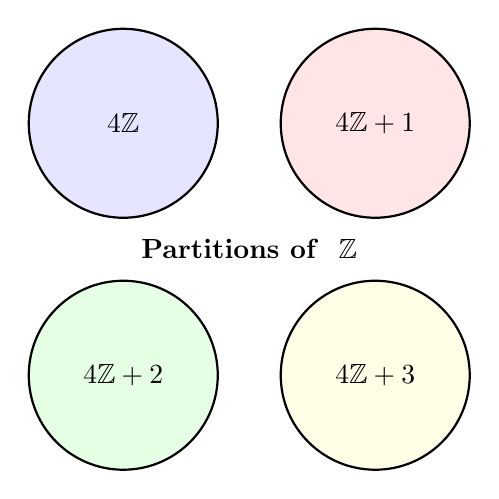
\begin{tikzpicture}[scale=0.8]
    \draw[thick, fill=blue!10] (0,0) circle (1.5cm) node {$4\mathbb{Z}$};
    \draw[thick, fill=red!10] (4,0) circle (1.5cm) node {$4\mathbb{Z}+1$};
    \draw[thick, fill=green!10] (0,-4) circle (1.5cm) node {$4\mathbb{Z}+2$};
    \draw[thick, fill=yellow!10] (4,-4) circle (1.5cm) node {$4\mathbb{Z}+3$};
    \node at (2, -2) {\textbf{Partitions of } $\mathbb{Z}$};
\end{tikzpicture}
\end{center}
\end{proof}

\subsection{Solution to Problem 28}
\begin{proof}
\textbf{Proof Technique: Probability Measure on Equivalence Classes.} \\
The sample space is $\Omega = \{1, 2, \dots, 1000\}$. The probability measure for a uniform distribution is $\mathbb{P}(A) = \frac{|A|}{|\Omega|}$.
The random variable $X(\omega) = \omega \bmod 5$ partitions $\Omega$ into 5 equivalence classes (events) based on the remainder when divided by 5: $E_0, E_1, E_2, E_3, E_4$.
Because 1000 is perfectly divisible by 5 ($1000 = 5 \times 200$), every contiguous block of 5 integers contains exactly one element from each equivalence class. There are exactly 200 such blocks.
Therefore, the cardinality of each event $E_i = \{\omega \in \Omega \mid X(\omega) = i\}$ is exactly 200.
\[ \mathbb{P}(X = i) = \frac{|E_i|}{|\Omega|} = \frac{200}{1000} = \frac{1}{5} = 0.2 \]
Since $\mathbb{P}(X = i) = 0.2$ for all $i \in \{0, 1, 2, 3, 4\}$, the probability distribution is perfectly uniform, meaning the data load is perfectly balanced across all 5 GPUs.
\end{proof}

\subsection{Solution to Problem 29}
\begin{proof}
\textbf{Proof Technique: Transitivity of Modular Congruence.} \\
Assume $T_1$ and $T_2$ are in the same bucket, and $T_2$ and $T_3$ are in the same bucket. By the definition of the buckets, this means:
\[ T_1 \equiv T_2 \pmod{\Delta t} \implies \Delta t \mid (T_1 - T_2) \]
\[ T_2 \equiv T_3 \pmod{\Delta t} \implies \Delta t \mid (T_2 - T_3) \]
By the definition of divisibility, there exist integers $k_1, k_2 \in \mathbb{Z}$ such that:
\[ T_1 - T_2 = k_1 \Delta t \]
\[ T_2 - T_3 = k_2 \Delta t \]
We wish to show $T_1$ and $T_3$ are in the same bucket, which requires $\Delta t \mid (T_1 - T_3)$. Adding the two equations yields:
\[ (T_1 - T_2) + (T_2 - T_3) = k_1 \Delta t + k_2 \Delta t \]
\[ T_1 - T_3 = \Delta t (k_1 + k_2) \]
Since $k_1 + k_2 \in \mathbb{Z}$, $\Delta t \mid (T_1 - T_3)$. Thus, $T_1 \equiv T_3 \pmod{\Delta t}$, meaning they belong to the same bucket.
\end{proof}

\subsection{Solution to Problem 30}
\begin{proof}
\textbf{Proof Technique: Synthesis of Parity, Modular Filters, and Coprime Divisibility.} \\
Let $p > 3$ be a prime number. We wish to prove $24 \mid (p^2 - 1)$. Note that $24 = 8 \times 3$. Since $\gcd(8, 3) = 1$, if we can prove $8 \mid (p^2 - 1)$ and $3 \mid (p^2 - 1)$, then by the theorem proven in Problem 17, $24 \mid (p^2 - 1)$.

\textbf{Step 1: Prove $8 \mid (p^2 - 1)$.}
Since $p$ is a prime strictly greater than 3, $p$ cannot be even (the only even prime is 2). Thus, $p$ is odd. By the result proven in Problem 7, if any integer $n$ is odd, $8 \mid (n^2 - 1)$. Therefore, $8 \mid (p^2 - 1)$.

\textbf{Step 2: Prove $3 \mid (p^2 - 1)$.}
Since $p$ is a prime strictly greater than 3, $p$ cannot be a multiple of 3 (the only prime multiple of 3 is 3 itself). Thus, $3 \nmid p$. By the result proven in Problem 15, if $3 \nmid p$, then $p^2 \equiv 1 \pmod 3$. This is equivalent to saying $3 \mid (p^2 - 1)$.

\textbf{Step 3: Synthesize.}
We have established that $8 \mid (p^2 - 1)$ and $3 \mid (p^2 - 1)$. Because $\gcd(8, 3) = 1$, their product must divide the target expression.
\[ (8 \times 3) \mid (p^2 - 1) \implies 24 \mid (p^2 - 1) \]
This completes the proof.
\end{proof}

\newpage

\section{Concept Checklist \& Question Mapping (Repeated)}
\label{sec:checklist_end}
For easy reference, here is the mapping of theoretical concepts to the generated problem set:

\begin{itemize}
    \item \textbf{C1: Direct Algebraic Manipulation \& Axioms of Divisibility} (Problems 1, 2, 3)
    \item \textbf{C2: Transitivity \& Linear Combinations} (Problems 4, 5)
    \item \textbf{C3: Biconditional Proofs ($\implies$ and $\impliedby$)} (Problems 6, 7)
    \item \textbf{C4: Proof by Cases / Division Algorithm} (Problems 8, 9, 10)
    \item \textbf{C5: Proof by Contrapositive \& De Morgan's Laws} (Problems 11, 12, 13)
    \item \textbf{C6: Parity Analysis of Products} (Problems 14, 15)
    \item \textbf{C7: Modular Arithmetic as a Filter (Squares mod 3, 4, 8)} (Problems 16, 17)
    \item \textbf{C8: B\'ezout's Identity \& Coprime Integers} (Problems 18, 19)
    \item \textbf{C9: Euclid's Lemma \& Prime Properties} (Problems 20, 21)
    \item \textbf{C10: Diagnostic Testing (Identifying Logical Flaws \& Fallacies)} (Problems 22, 23, 24, 25)
    \item \textbf{C11: Set-Theoretic Partitions \& Equivalence Relations} (Problems 26, 27)
    \item \textbf{C12: Abstract Real-World Modeling (Probability, ML, Quant Finance)} (Problems 28, 29)
    \item \textbf{C13: Advanced Conceptual Synthesis} (Problem 30)
\end{itemize}

\end{document}